\documentclass{article}
\usepackage[utf8]{inputenc}
\usepackage{hyperref}
\usepackage{graphicx}

\hypersetup{
    colorlinks=true,
    linkcolor=blue,
    filecolor=magenta,      
    urlcolor=cyan,
    pdftitle={Sharelatex Example},
    bookmarks=true,
    pdfpagemode=FullScreen,
    }

\title{Learning Journal: Week 9-13}
\author{Sophie Avard}
\date{October 2019}

\begin{document}

\maketitle

\section{Introduction}



\section{User Story 4}
\subsection{Intention}
Add a tool to Zotero to automatically add files library.

\subsection{Action}
\begin{enumerate}
    \item Go to Chrome Web Store and search for Zotero 
    \item Click the 'add to Chrome' button 
    \item Login via the connector using my Zotero account
    \item Click pdf button on top right of screen to save metadata and pdf straight into Zotero
\end{enumerate}
\subsection{Error}
No error but it is hard to locate PDF's when downloaded as the file name is often hard to read. 

\section{User Sotry 4}
\subsection{Intention}
Add a tool to Zotero to automatically change the name of the PDF's.
\subsection{Action}
\begin{enumerate}
    \item Install ZotFile: \href{http://zotfile.com/#features}{http://zotfile.com/features}  
    \item In Zotero go to tools - Add-ons - Tools for all Add-ons - Install Add-on from file - selection the downloaded .xpi file
    \item Change the source folder for attaching new files: Tools - ZotFile Preferences - set to User/sophieavard/Downloads
    \item In Renaming Rule tab: Click 'use Zotero to rename' and format item types as: \verb|author lastname_year_title| (see image below)
\end{enumerate}
   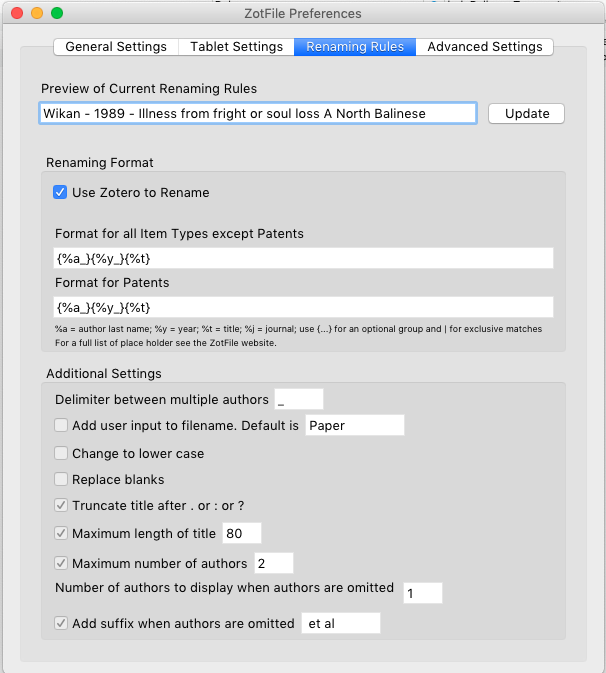
\includegraphics[width=12cm]{zotfile.png}
\subsection{Error}
NA. 
\section{User Story 2}
\subsection{Intention}
Retrieve metadata from Zotero in a report format. 
\subsection{Action}
\begin{enumerate}
\item Select items to be included in metadata report
\item Right click - click 'generate report for items' 
\end{enumerate}
\subsection{Error}
No error but report isn't very flexible. Doesn't allow me to edit the metadata. 

\section{User Story 2}
\subsection{Intention}
Add a tool to help make metadata report more flexible. 
\subsection{Action}
\begin{enumerate}
    \item Download Report Customiser for Zotero: \href{https://github.com/retorquere/zotero-report-customizer}{Zotero Report Customiser}
    \item In Zotero click toools - Add-ons - Extensions
    \item Click on the gear in the top-right and choose 'install add-on from file'
    \item Choose the .xpi that was just downloaded and click 'Install'
    \item Re-start Zotero
\end{enumerate}
Produce report:
\begin{enumerate}
    \item Select items to be included in report
    \item right click - click 'generate report for items' 
    \item Click edit button in top left corner 
    \item Edit metadata report (See image below)
\end{enumerate}
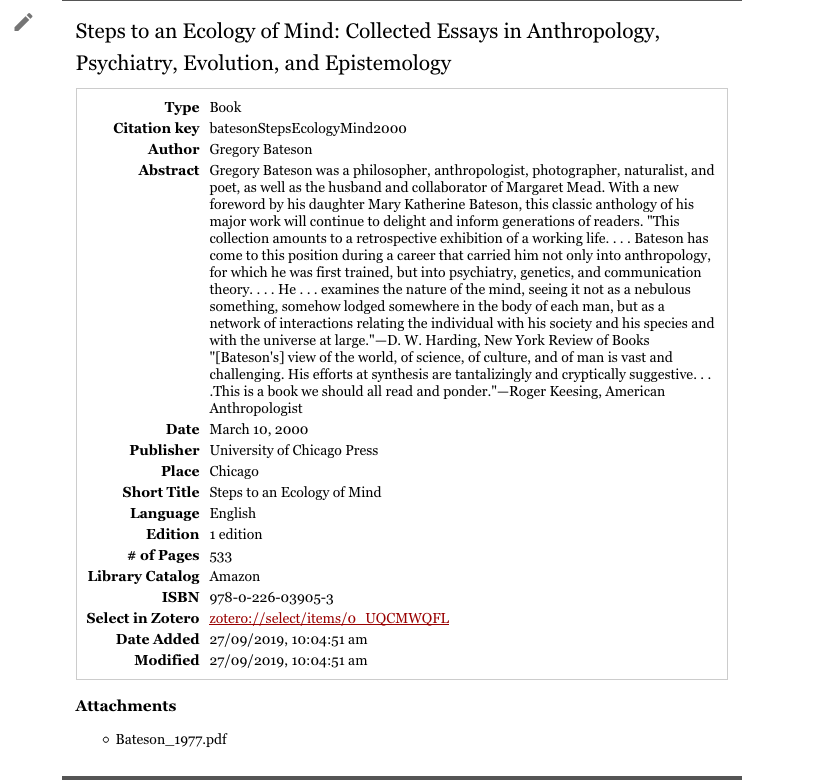
\includegraphics[width=12cm]{metadata.png}

\section{User Story 8}
\subsection{Intention}
Produce a table/graph to help draw connections and relationships between items. Download ZotNet tool to allow me to see relationships and calculate basic statistics. \\
\textbf{ZotNet}: \href{https://www.exitsantacruz.com/zotnet/zotnet.php}{https://www.exitsantacruz.com/zotnet/zotnet.php}
\subsection{Action}
\begin{enumerate}
    \item Download NetDraw to open Zotnet analysis: \href{https://sites.google.com/site/netdrawsoftware/home}{NetDraw}
    \item Click 'Installation Package'
    \item Follow the prompts on the screen 
\end{enumerate}
\subsection{Error}
Download didn't work.

\section{User Story 8}
\section{Intention}
Download and install UCINET which will automatically install NetDraw.
\section{Action}
\begin{enumerate}
    \item Go to: \href{https://sites.google.com/site/netdrawsoftware/home}{NetDraw}
    \item Click UCINET
    \item Download 32-bit Installation package 
    \item Read installation notes at bottom
\end{enumerate}
\section{Error}
Installation notes state that UCINET cannot be run on Mac. Need to use a Windows emulator to run UCINET. 

\section{User Story 8}
\subsection{Intention}
Download Wine for mac so that I can run UCINET on my Mac. 
\subsection{Action}
\begin{enumerate}
\item Download UCINET and save to Desktop. The url for this is: \href{https://sites.google.com/site/ucinetsoftware/downloads}{UCINET Software}
\item Install X11: Go to \href{https://www.xquartz.org}{XQuartz} and download the latest version. 
    \item Download: \href{http://winebottler.kronenberg.org}{WineBottler1.7.37} 
    \item Follow installation prompts then add Wine and WineBottle into Applications folder.
\end{enumerate}
To Run WineBottle:
\begin{enumerate}
    \item Find WineBottle in Applications
    \item Go to 'Advanced' and under 'Program Installation' click 'select file'
\end{enumerate}
\section{Error}
WineBottle unexpectedly closed and this error message appeared:\\
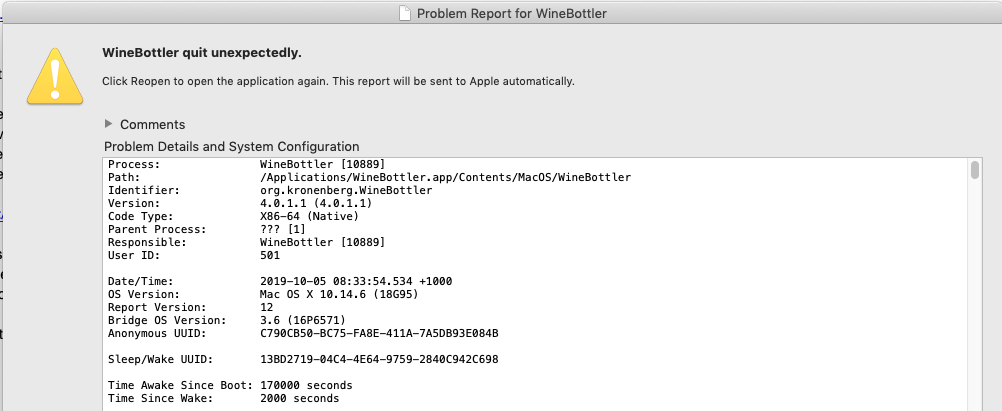
\includegraphics[width=12cm]{WineBottle.png}

\section{User Story 8}
\subsection{Intention}
Download Version 1.8.6 of WineBottle to see if it works.

\subsection{Action}
\begin{enumerate}
    \item Go to: \href{http://winebottler.kronenberg.org}{http://winebottler.kronenberg.org}
    \item Click 'Winebottler 1.8.6 Stable'
    \item Click 'Skip Ad' in top right corner 
    \item Once installed, add Wine and WineBottler to Applications
\end{enumerate}
Try to run WineBottler:
\begin{enumerate}
    \item Open spotlight - search WineBottler 
    \item Click the application and then click 'Advanced' 
    \item Under 'Program Installation' click 'selection file' and select 'Setup32UCI6685.exe' on Desktop
    \item Under 'Winetricks' search 'mdac28' and select it.
    \item Click install and follow prompts
    \item Once installation is finished it asks which file is my 'Startfile' - select 'Program Files/Analytic Technologies/Uci6.exe'
\end{enumerate}
\section{Error}
Still can't open NetDraw.

\section{User Story 8}
\subsection{Intention}
Try use to Paper Machines add-on instead. Link here: \href{http://papermachines.org/install/}{Paper Machines}

\subsection{Action}
\begin{enumerate}
    \item Click the link to install 
    \item Open Zotero
    \item Click tools - add-ons - install new add on from file 
    \item Click Paper Machine download
\end{enumerate}

\subsection{Error}
Got error message. Did not work. 

\section{User Story 8}
\section{Intention}
See if Zotero Voyant export tool can visualise connections and relationships. Note, VoyantServer allows you to handle large texts without the connection timing out. 

\section{Action}
Link: \href{http://docs.voyant-tools.org/resources/run-your-own/voyant-server/}{Voyant Export}
\begin{enumerate}
    \item Download Java
    \item Download VoyantServer.zip file 
    \item Run server by double clicking on download
    \item Voyant control panel will appear (see image below)
\end{enumerate}
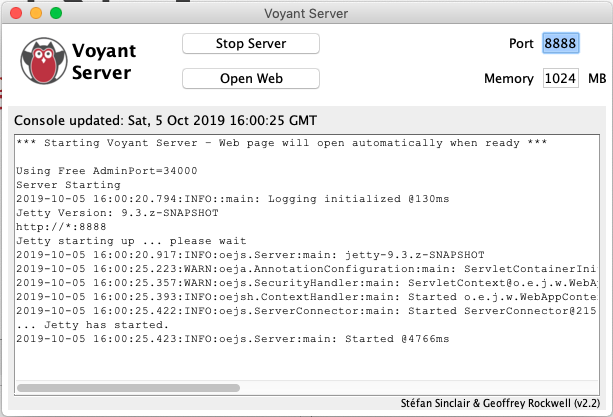
\includegraphics[width=12cm]{voyantserver.png}

\begin{enumerate}
    \item VoyantServer will automatically launch in browser. 
    \item Right click on collection then click 'export collection to voyant'
    \item Save zip file to desktop as 'Bali.zip'
    \item Open Voyant and upload Bali.zip file to Voyant. 
\end{enumerate}
NOTE: List of Voyant tools: \href{https://voyant-tools.org/docs/#!/guide/tools}{Here}\\
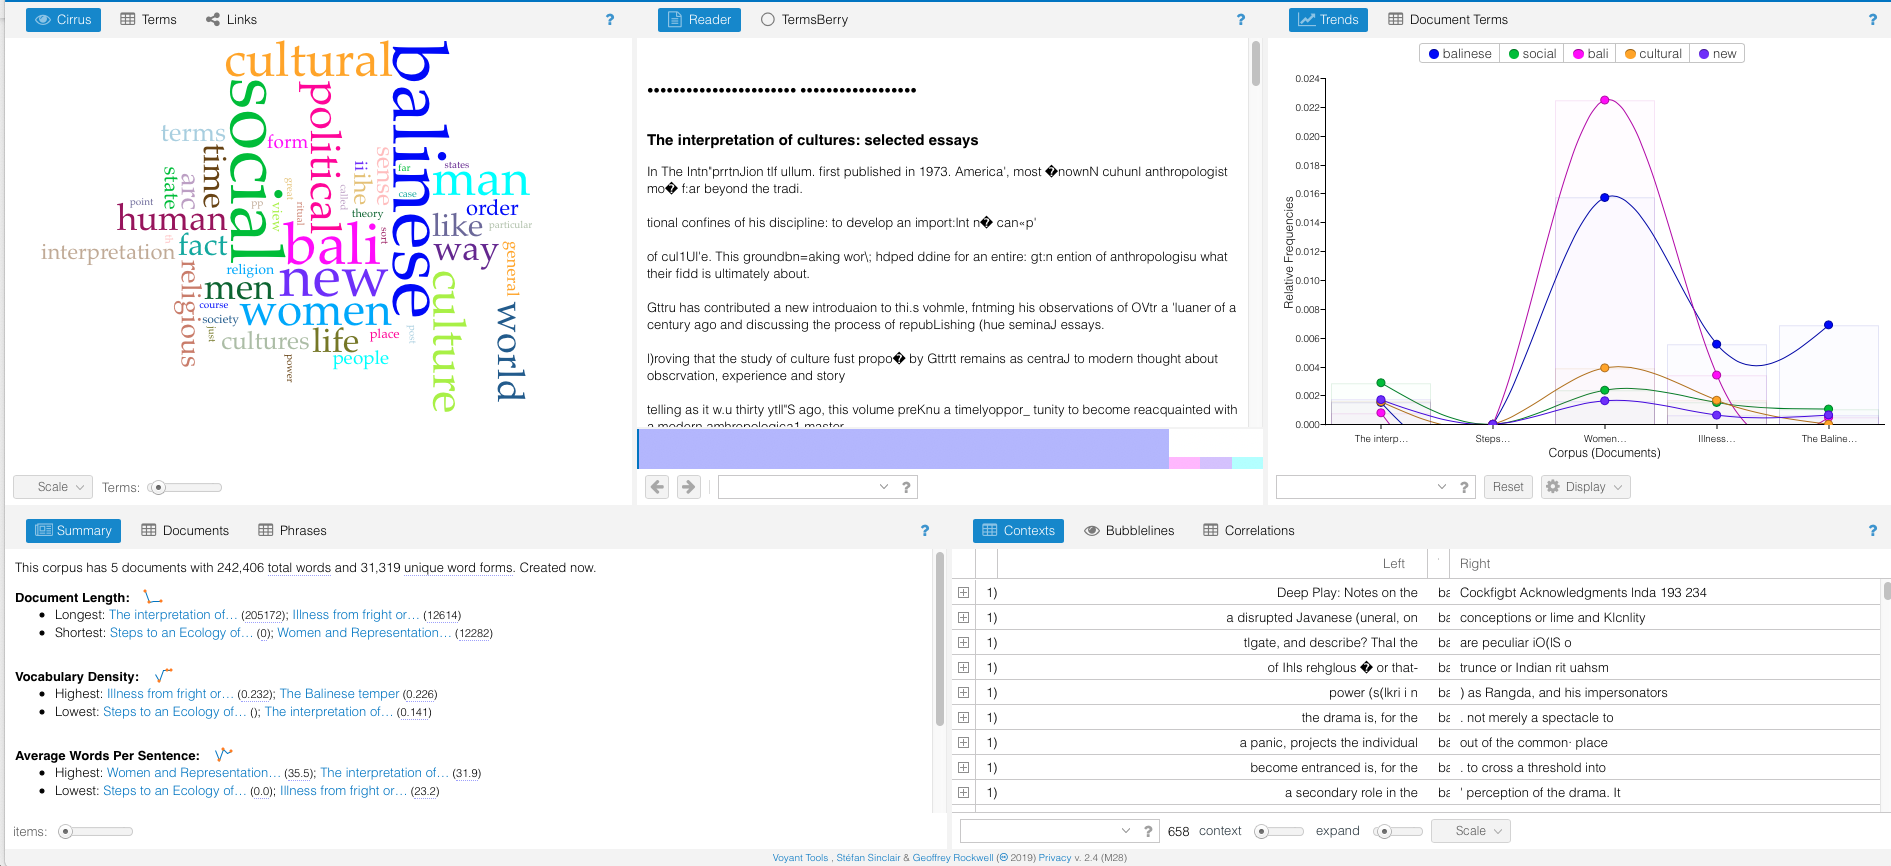
\includegraphics[width=15cm]{voyant.png}

\subsection{Error}
None.

\section{Hypothes.is}
\subsection{Intention}
Text Hypothes.is to see if it is better than Voyant.
\subsection{Action}
\begin{itemize}
    \item Go to Hypothes.is website
    \item Create login
    \item Upload pdf 
    \item highlight pdf 
    \item annotate pdf
    \item save 
\end{itemize}
\subsection{Error}
No error but looks difficult to export. Exporting is not essential for PoC but would be useful. After doing some research apparently you can import annotations into OpenSemantic Desktop Search. 

\section{Following meeting with Brian}
\subsection{Intention}
Try to use OpenSemantics for searching texts and tagging. 
\subsection{Action}
\begin{enumerate}
    \item Download VirtualBox: \href{https://www.virtualbox.org}{https://www.virtualbox.org}
    \item Download OpenSemantics.org: \href{https://www.opensemanticsearch.org}{https://www.opensemanticsearch.org}
    \item Open VirtualBox 
    \item Click import 
    \item Select OpenSemantics file 
    \item Double click OpenSemantics 
\end{enumerate}
\subsection{Error}
When I tried to launch OpenSemantic I got a message saying that I needed a login and password. 

\section{OpenSemantic Desktop Search }
\subsection{Intention}
Attempt to fix previous error by re-downloading and following the manual again.
\subsection{Action}
\begin{enumerate}
    \item Open VirtualBox
    \item Download \verb|open-semantic-desktop-search_19.07.19.ova|: \href{https://www.opensemanticsearch.org}{https://www.opensemanticsearch.org}
    \item Start VirtualBox 
    \item Click 'file'
    \item Click 'import appliance'
    \item Choose the downloaded open-semantic-desktop-search file.
    \item Click settings 
    \item Click shared folders 
    \item select folder with relevant files
    \item double click OpenSemantic on left panel to start
\end{enumerate}
\subsection{Error}
No error but tool ran extremely slowly. I Googled it and apparently VirtualBox is slow.

\section{OpenSemantic Desktop Search}
\subsection{Intention}
Make sure that it can:
\begin{itemize}
    \item Tag sources
    \item Search Sources
    \item Import from Hypothes.is
\end{itemize}
\subsection{Action}
\begin{enumerate}
    \item Open VirtualBox
    \item Make sure shared folder is the folder that contains my sources
    \item Launch OpenSemantic 
    \item Click on annotations and tagging 
    \item add tag 
    \item save (successful)
    \item Go back to home page 
    \item Click search
    \item Search for word 'stress' (successful)
    \item Go to Datasource 
    \item Click Hypothesis
    \item Click import
    \item Go to Hypothes.is website \href{https://hypothes.is}{https://hypothes.is}
    \item Click Settings
    \item Click Developer
    \item Copy API token
    \item Go back to OpenSemantic
    \item Paste API token 
    \item Click import
\end{enumerate}
Note: more detailed steps are outlined in PoC Design.
\subsection{Error}
OpenSemantic seems to be able to successful search, tag and import from Hypothes.is. While there were no errors, the automatic tagging seemed to pick up the wrong words. Next time I will convert a pdf to .txt file to see if OpenSemantic is more efficient.

\section{QCoder}
\subsection{Intention}
Run through a quick elaboration of QCoder on R to see if it is better than OpenSemantic Search. Link: \href{https://github.com/ropenscilabs/qcoder}{https://github.com/ropenscilabs/qcoder}

\subsection{Action}
Conduct test with some sample data:

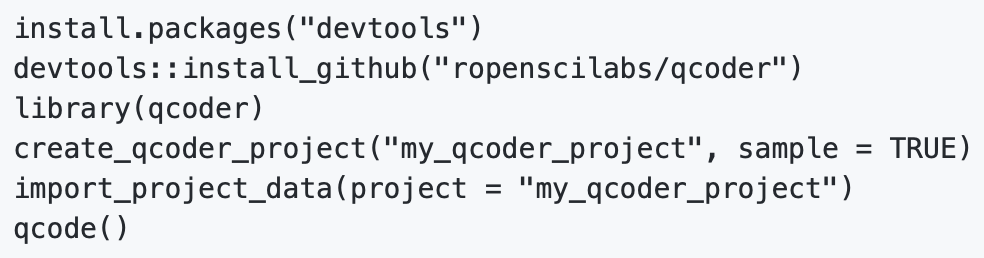
\includegraphics[width=10cm]{QCoder.png}

Then select 'project folder' and my qcoder project'. Highlight the text and select 'add code' then 'save changes'. Export csv file to make sure that is shows coded literature and the document that it came from. 

Coding works well - Maybe try to link Voyant with it to export most frequently used words as codes. 

\subsection{Error}
No error with sample data. Now need to try my own data. 

\section{Text QCoder with my data}
\subsection{Intention}
Add 3 text files of my own data to RCoder and see if it works.
\subsection{Action}
Code and coding below - test was successful.

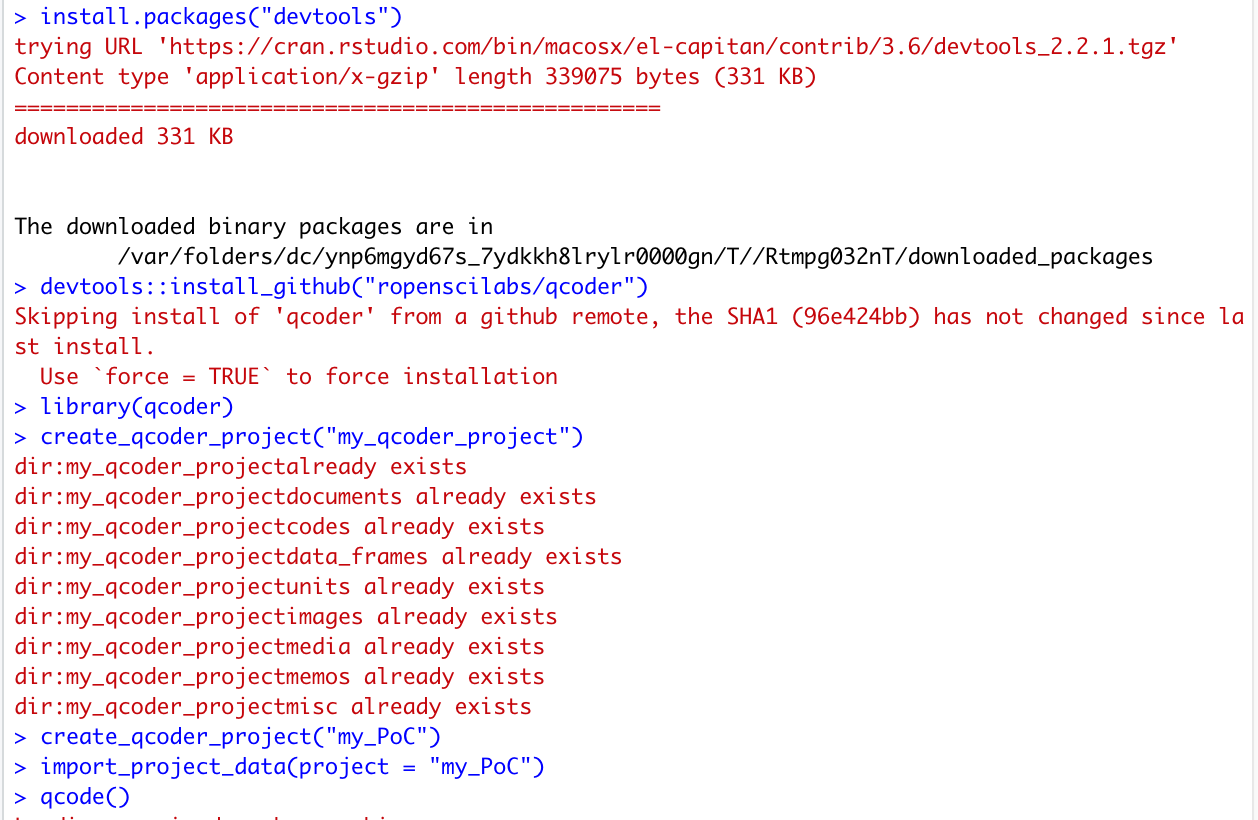
\includegraphics[width=10cm]{QCoder2.png}

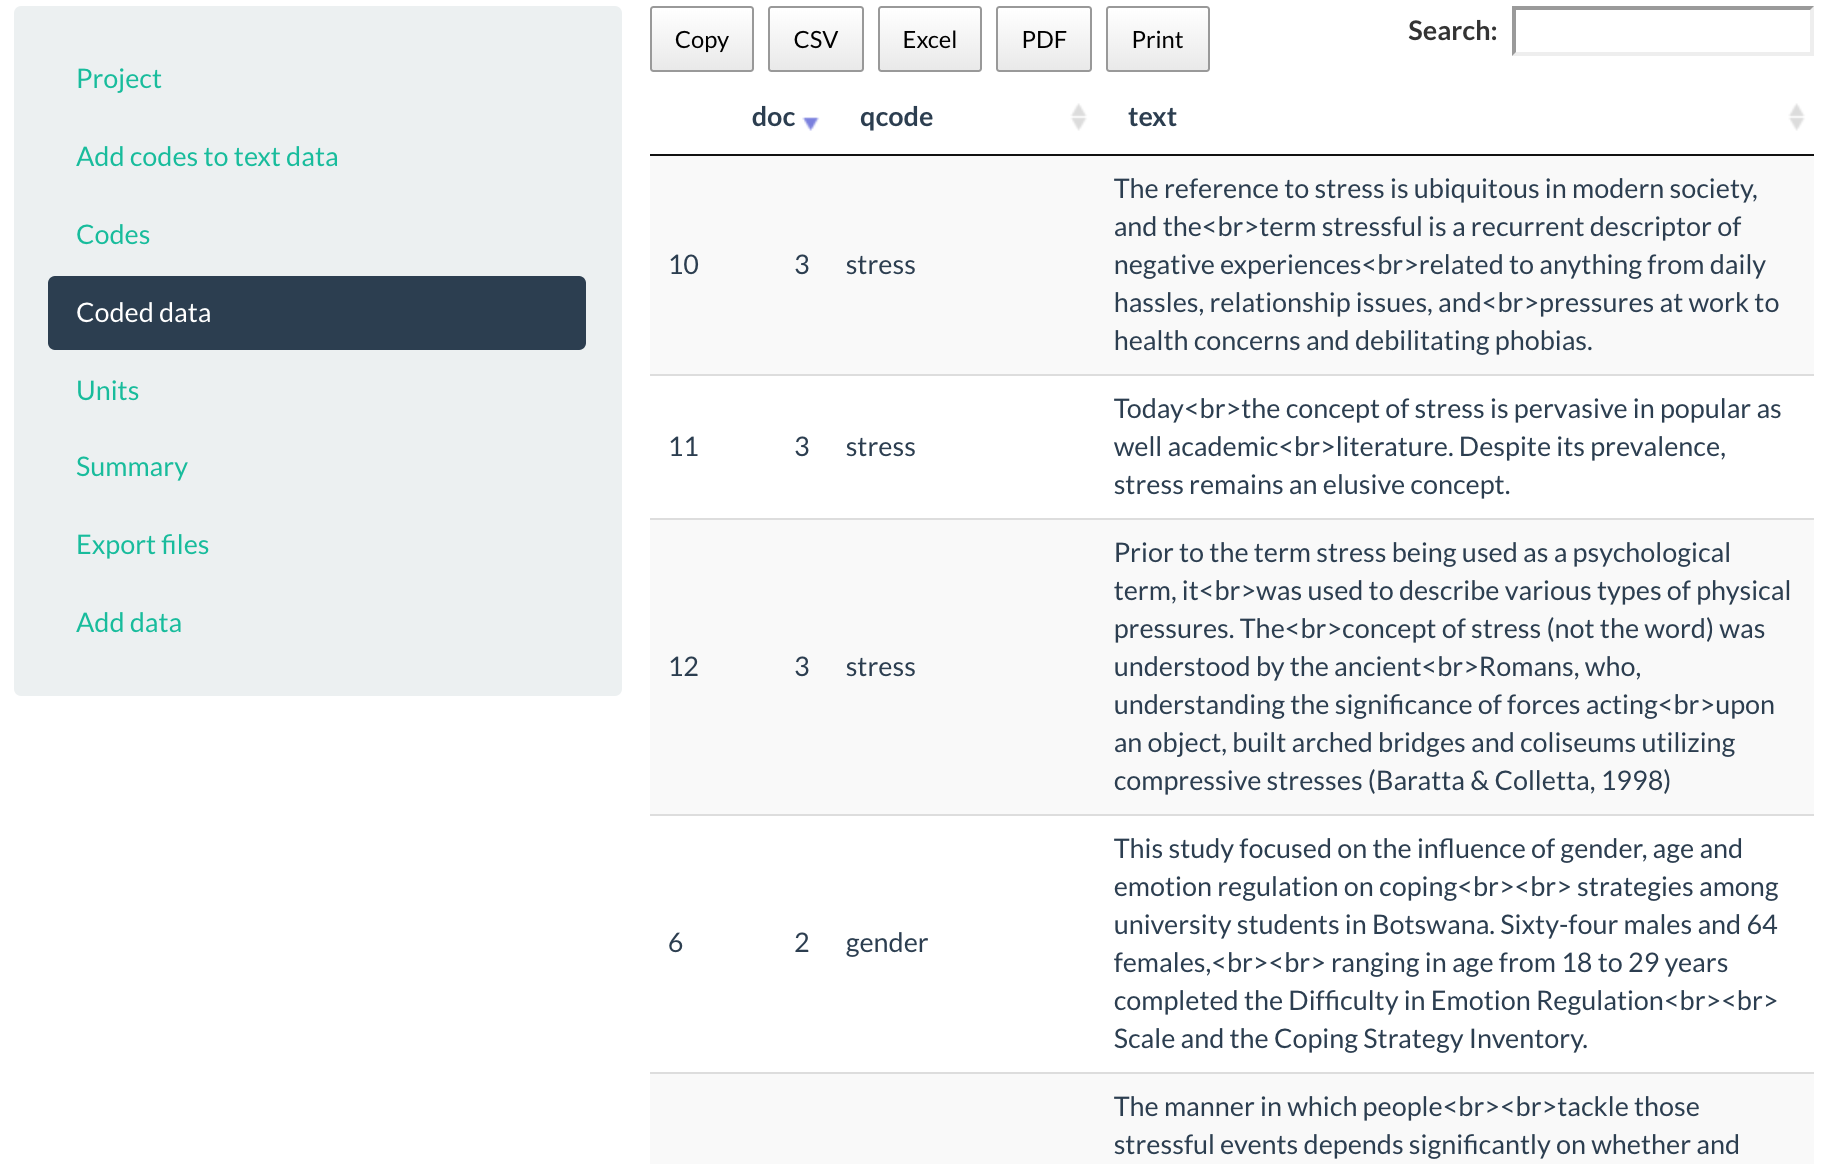
\includegraphics[width=10cm]{QCoder_coded.png}

\subsection{Error}
No error but \verb|<br>| appeared in the 'text' after items were coded. See if OpenRefine can clean the csv file.

\section{OpenRefine}

\subsection{Intention}
Use OpenRefine to clean analysis produced by coding.

\subsection{Action}
\begin{enumerate}
    \item Rename columns to Source, Code and Text 
    \item Clean the text column to remove \verb|<br>| 
    \item Extract Operation History for later use by clicking 'undo/redo' - extract - then copy the script into a text file and save it to Desktop.
\end{enumerate}

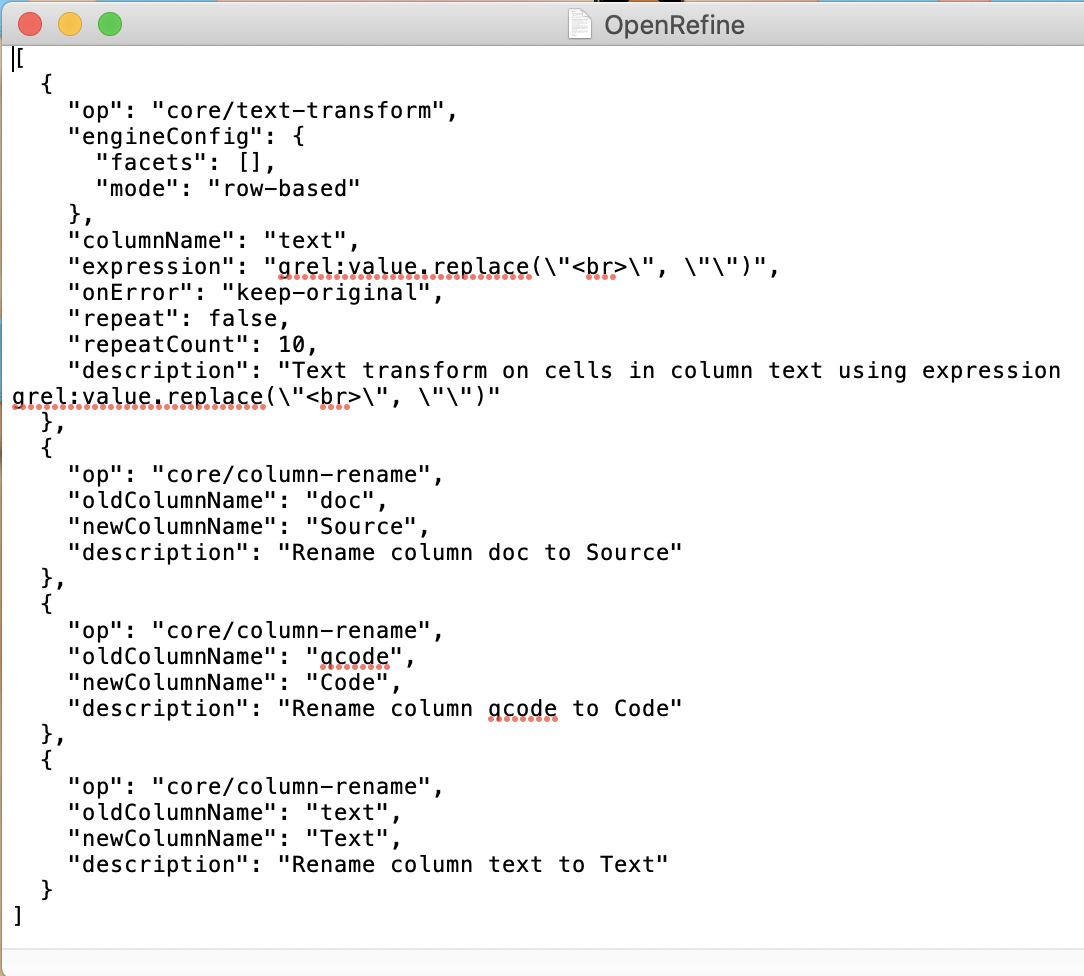
\includegraphics[width=10cm]{openrefine.png}

\subsection{Error}
No error - followed instructions from class. 

\section{pdf to text file}
\subsection{Intention}
Write command in mac terminal to coonvert pdf to text file.

\subsection{Action}
Instructions: \href{https://apple.stackexchange.com/questions/155250/trying-to-convert-pdf-to-text-for-free}{https://apple.stackexchange.com/questions/155250/trying-to-convert-pdf-to-text-for-free}

Below is a screenshot of the code that I wrote to convert a pdf document to a text file. 

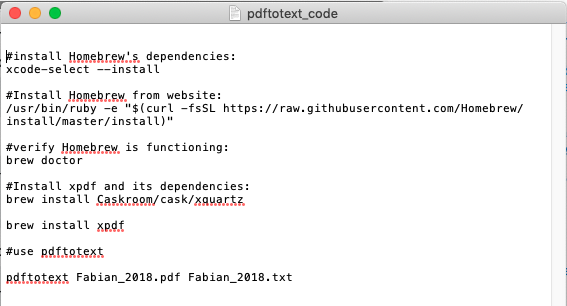
\includegraphics[width=12cm]{pdftotext.png}

\subsection{Error}
I did not use cd to navigate to the directory that the pdf was in - so when I tried to use the pdftotext command it could not open the file. I then used cd to navigate to my Desktop and tried again. It successful saved a text file to my Desktop called \verb|'Fabian_2018.txt'|

\section{Loop pdftotext command}
\subsection{Intention}
Use instructions on Unix Shell to loop pdftotext command for 3 documents
\subsection{Action}
Below is the command that I used:

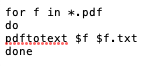
\includegraphics[width=5cm]{pdftotextloop.png}

\subsection{Error}
The first time I tried to run the command I inserted ./ before 'pdftotext'. I then got an error message. 

\section{Move converted pdf's into different location}
\subsection{Intention}
Now that I have a command to convert pdf's to text, I want to be able to move all converted pdf's into a few folder. 

\subsection{Action}
Add mv command into loop to move all pdf's into a folder called converted. See command below:

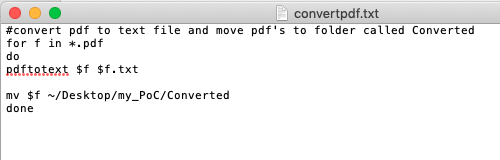
\includegraphics[width=10cm]{converted.png}

\subsection{Error}
No error. 

\section{Change name of files}
\subsection{Intention}
Change the name of the files using a csv files.

\subsection{Action}
\begin{enumerate}
    \item Create a excel spreadsheet
    \item Save it as myfiles
    \item for each row add \verb|"file_name"|,\verb|"new_file_name"|
\end{enumerate}
Use this script to run a test to see the output:

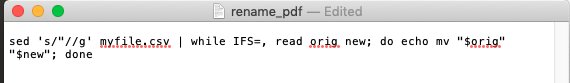
\includegraphics[width=10cm]{echo_rename.png}

Output looks correct, terminal shows that the script will use the 'mv' command to re-name particular files (see below).

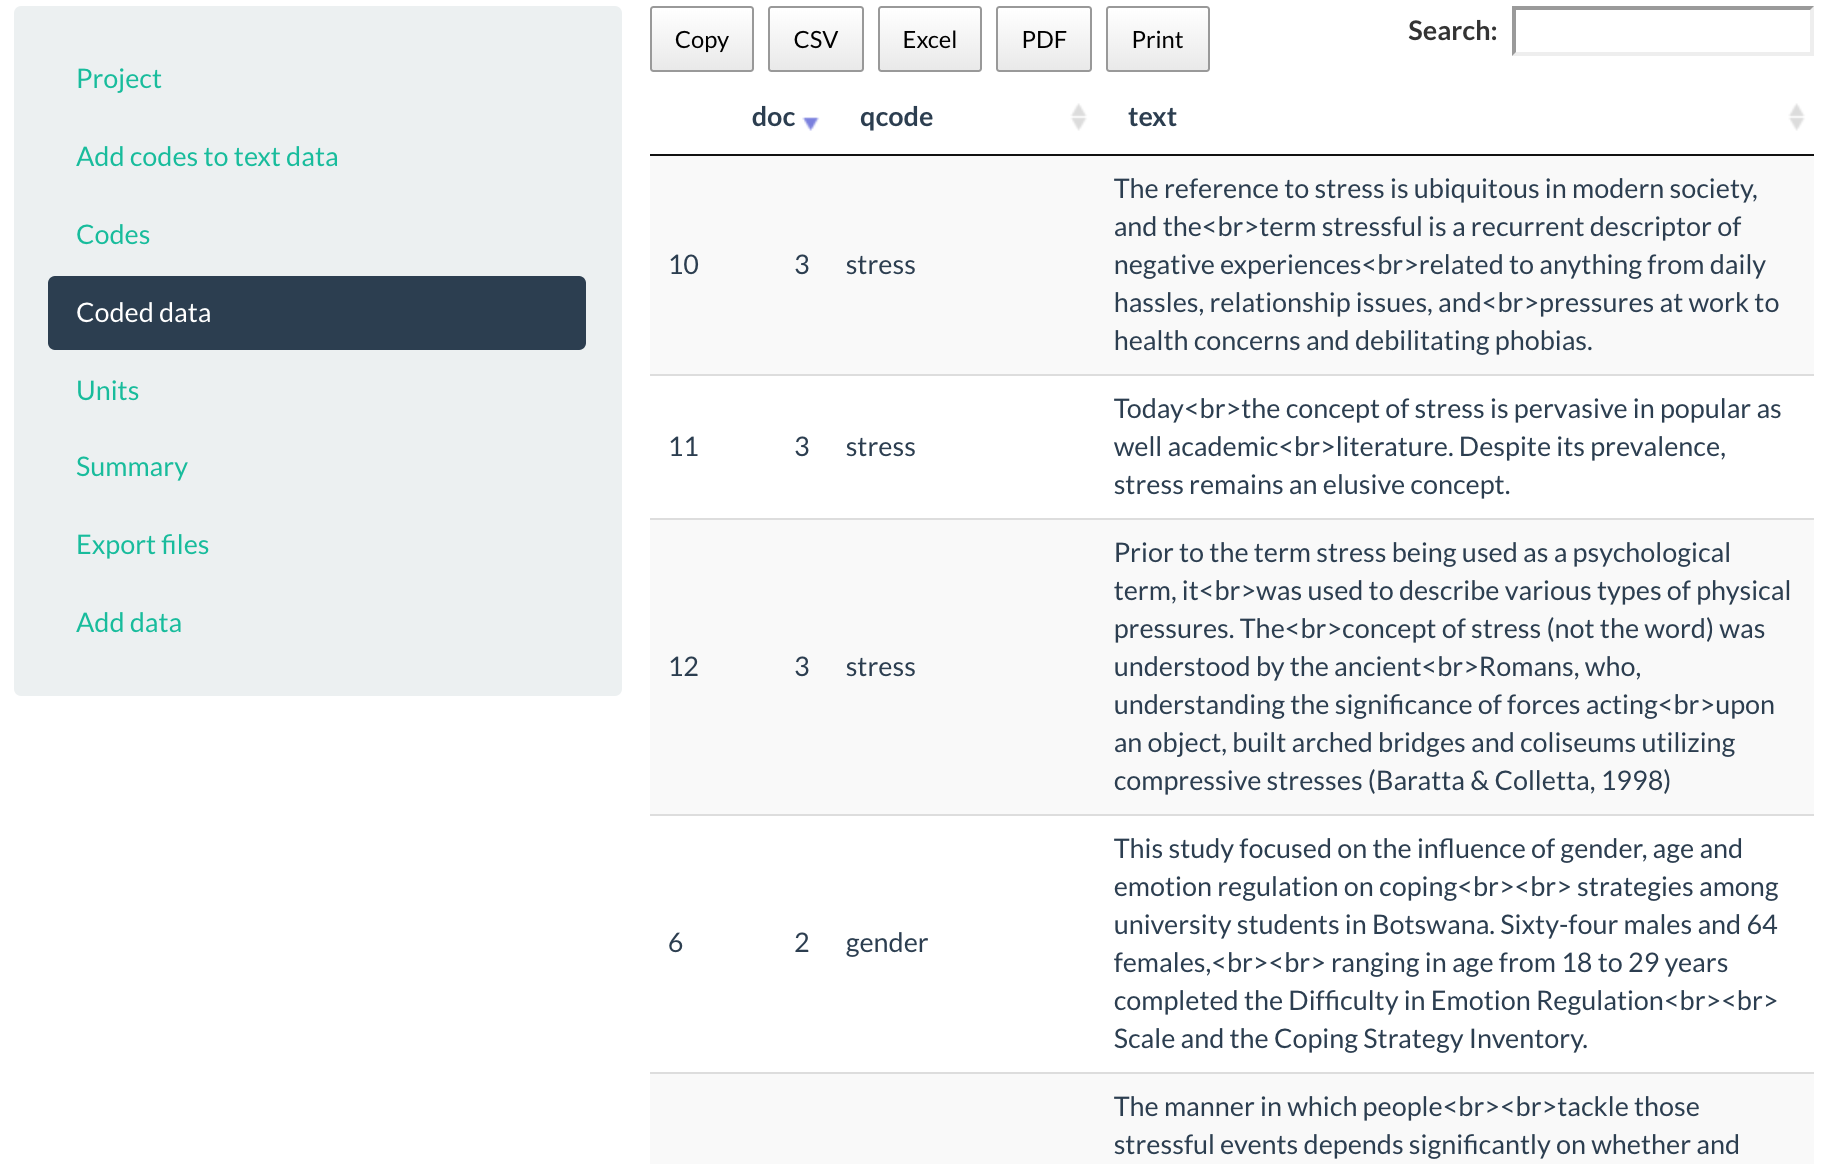
\includegraphics[width=10cm]{test.png}

Now, change file names by removing 'echo' command from the above script.

\subsection{Error}
The echo command successfully showed that the files would be renamed. However, when removing 'echo' and trying to run the script it said that
\verb|'rename My Heart Die in Me.pdf to Fabian_2018.pdf\r: No such file or directory'|

\section{Introduction to R}

\subsection{Intention}
Complete the exercise - What do you think is the current content of the object area acres? 

\subsection{Action}
I think that it will remain as 6.175.

\subsection{Error}
None.

\subsection{Intention}
Complete the exercise - create two variables (length and width) and assign them values. Add third variable (area) and give it a value based on the current values.

\subsection{Action}
I followed the steps in the exercise on data carpentry. Although I got different results.

\subsection{Error}
First error: I accidentally clicked the wrong key on my keyboard - R came back with an error message so I retyped it.

Second error: the value of the area should have been 8 and I got 6.26=5
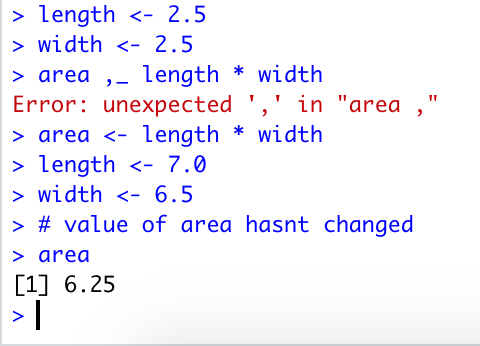
\includegraphics[width=10cm]{length_width.png}

\subsection{Intention}
Exercise - Type ?round at the console and then look at the output in the Help pane. What other functions exist that are similar to round? How do you use the digits parameter in the round function?

\subsection{Action}
\begin{enumerate}
    \item Ceiling - takes a single numeric argument x and returns a numeric vector containing the smallest integers not less than the corresponding element of x
    \item Floor - returns a numeric vector containing the largest integers not greater than the corresponding elements of x
    \item Trunc - returns a numeric vector containing the integers formed by truncating the values in x toward 0
    \item Signif - rounds the values in its first argument to the specified number of significant digits
\end{enumerate}

\subsection{Error}
NA

\subsection{Intention}
Exercise - what happens if we try to mix these types in a single vector?

\subsection{Action}
R converts them to all be the same type. Vectors can only be one data type.

\subsection{Error}
I had no clue what it was talking about - had to look at the solutions..

\subsection{Intention}
1. Using the vector of rooms, create a new vector with the NAs removed
2. Use the function median() to calculate the median of the rooms vector 
3. Use R to figure out how many households in the set use more than 2 rooms for sleeping

\subsection{Action}
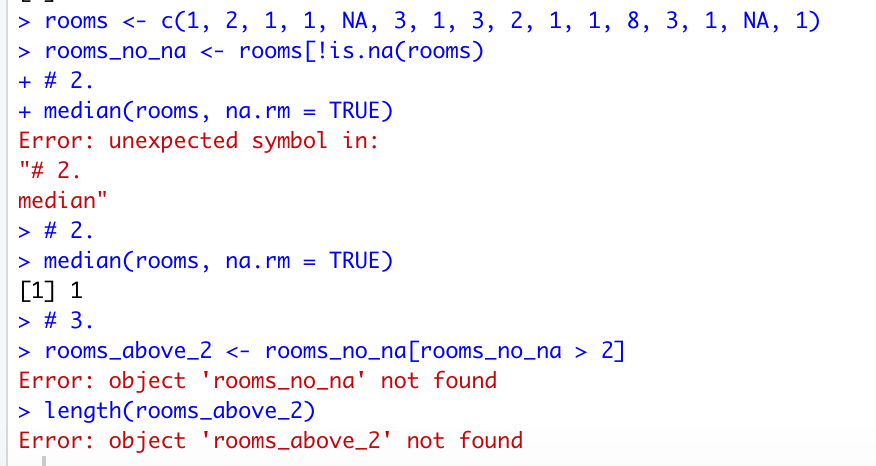
\includegraphics[width=12cm]{rooms.png}

\subsection{Error}
As can be seen above, there were multiple errors in this exercise. However, I just followed the instructions, dont understand why the object wasnt found

\section{Starting with Data}

\subsection{Intention}
Complete the exercise: 
1. Create a data frame containing only the data in row 100 of the interviews dataset
2. notice how nrow() gave you the number of rows in a data frame.
3. use nrow() to extract the row that is in the middle of the data frame.
4. combine nrow() with the - notation above to reproduce the behaviour of head(interviews)


\subsection{Action}
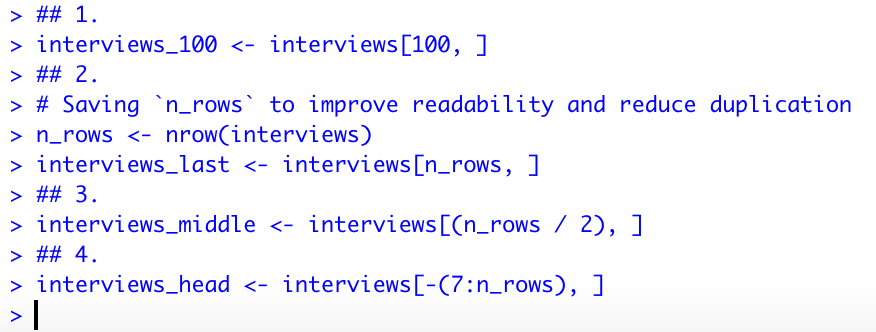
\includegraphics[width=12cm]{nrow.png}

\subsection{Error}
I was very lost with this exercise - I had to follow the solution. Dont really understand how this is useful for anthropological research.

\subsection{Intention}
Exercise - rename the levels of the factor to have the first letter in uppercase: "no", "undetermined", and "yes". Now recreate the barplot such that undetermined is last

\subsection{Action}
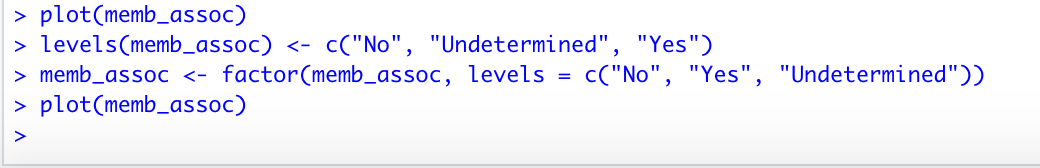
\includegraphics[width=12cm]{undetermined.png}

\subsection{Error}
NA

\section{Introducing dplyr and tidyr}

\subsection{Intention}
Exercise - using pipes, subset the interviews data to include interviews where respondents were members of an irrigation association and retain only the columns affect conflicts, liv count and no meals 

\subsection{Action}
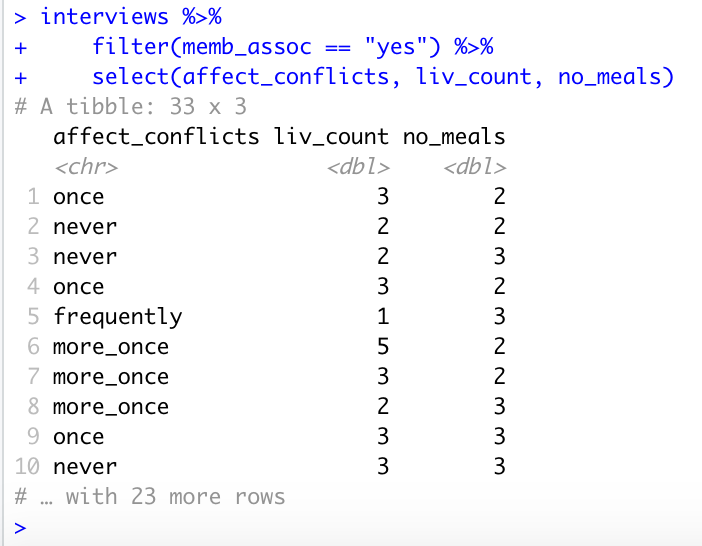
\includegraphics[width=12cm]{pipes.png}

\subsection{Error}
No error. But pipes might be useful for PoC if I can learn how to apply them to different packages.

\subsection{Intention}
Exercise - Create a new data frame from the interviews data that meets the following criteria: contains only the village column and a new column called total meals containing a value that is equal to the total number of meals served in the household per day on average. Only the rows where total meals is greater than 20 should be shown in the final data frame.

\subsection{Action}
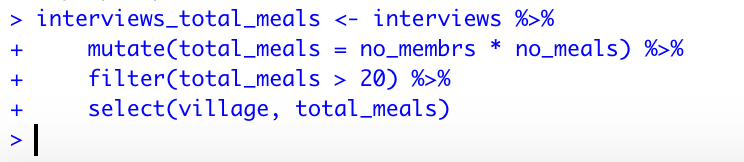
\includegraphics[width=12cm]{mutate.png}

\subsection{Error}
NA

\subsection{Intention}
Exercise - how many households in the survey have an average of two meals per day? three meals per day? are there any other numbers of meals represented? 

\subsection{Action}
Answer: 2 = 52, 3 = 79. No 

\subsection{Error}
None. 

\subsection{Intention}
Exercise - Create a new data frame that has one column for each month and records TRUE or FALSE for whether each interview respondent was lacking food in that month.

How many months were respondents without food if they did belong to an irrigation association? What about if they didnt?

\subsection{Action}
Answer: 2.64 and 2.31

\subsection{Error}
Not sure if my answer is correct.

\section{Data Visualisation with ggplot2}

\subsection{Intention}
Create a scatter plot of rooms by village with the respondent wall type showing in different colours.

\subsection{Action}
Cant really tell the different villages apart.\\
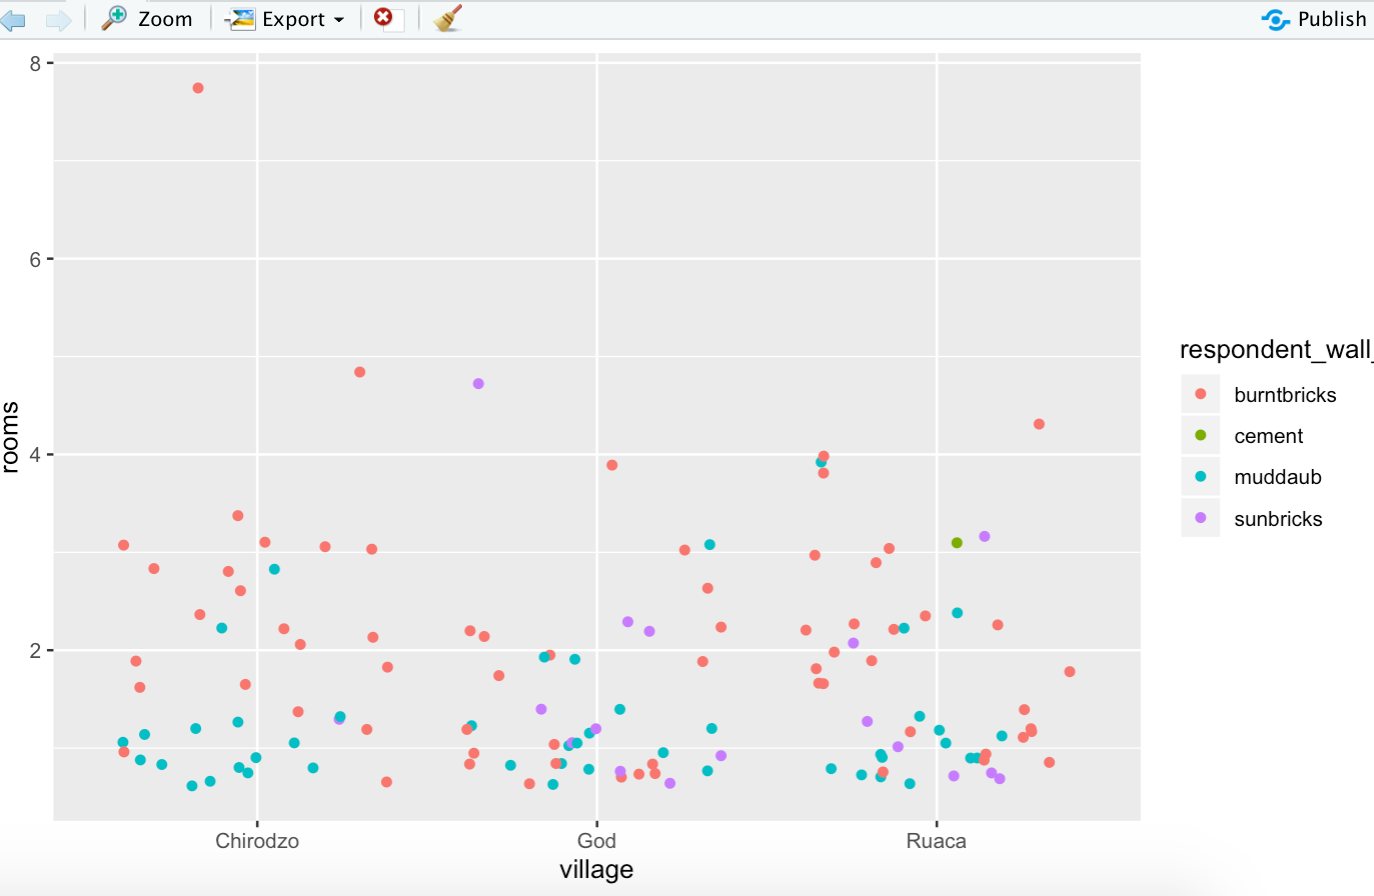
\includegraphics[width=10cm]{plot.png}

\subsection{Error}
None.

\subsection{Intention}
Boxplots are useful summaries, but hide the shape of the distribution. For example, if the distribution is bimodal, we would not see it in a boxplot. An alternative to the boxplot is the violin plot, where the shape (of the density of points) is drawn. Replace the box plot with a violin plot

\subsection{Action}

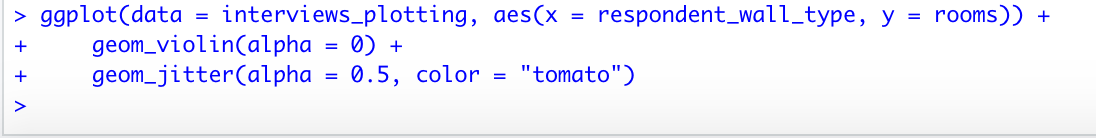
\includegraphics[width=10cm]{geom_violin.png}

\subsection{Error}
None.

\subsection{Intention}
Create a bar plot showing the proportion of respondents in each village who are or are not part of an irrigation association (memb assoc). Include only respondents who answered that question in the calculations and plot. Which village had the lowest proportion of respondents in an irrigation association?

\subsection{Action}
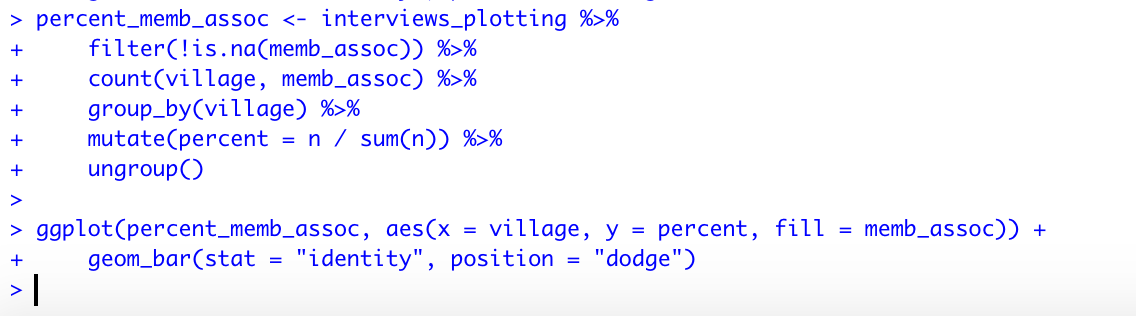
\includegraphics[width=10cm]{bar_plot.png}

\subsection{Error}
None.

\subsection{Intention}



\end{document}
